\chapter{State of the art}
\label{ch2}

%%%%%%%%%%%%%%%%%%%%%%%%%%%%%%%%%%%%%%%
% IMPORTANT
\begin{spacing}{1.25} %THESE FOUR
\minitoc % LINES MUST APPEAR IN
\end{spacing} % EVERY
\onehalfspacing % CHAPTER
% COPY THEM IN ANY NEW CHAPTER
%%%%%%%%%%%%%%%%%%%%%%%%%%%%%%%%%%%%%%%

\section{Riveted connection}

Before the development of welding technology and \ac{HSB}, rivets were commonly used to join steel structures. In particular, steel bridges built between 1860 and 1950 were almost exclusively riveted. In Japan, the era of cast iron began in 1897 and gave way to the era of steel. Until the introduction of welding in the 1950, riveted joints were used with 40 kg class structural steel (SS39A, SS41)\cite{rivet1934}. This oldest type of joint allows two or more metal sheets to be joined together. After being heated to a high temperature, the rivets are placed in the hole and a pneumatic hammer is used to form the other head. The rivet is then cooled to create a residual clamping force, thus realising the riveted joint.\footnote{this is foot note}

However, riveting requires skilled techniques and has problems and hazards such as noise and fire, so it is rarely used for new structures and is no longer described in the Road and Bridge Specifications after 1980. Welding, on the other hand, became the main method of fabricating members in factories around 1955 due to advances in welding technology and economic efficiency. Rivets also ceased to be used on site around 1965 due to a reduction in the number of riveters and noise problems, and were replaced by high-strength bolts.

Steel riveted bridges have significant cultural and historical value as part of our constructive heritage from the previous century. Numerous iron and steel riveted bridges are of historical importance, requiring restoration and preservation, and ongoing use. A large number of riveted bridges have been rebuilt due to age and corrosion, but many riveted bridges are still in service \cite{COLLETTE2014}. Most of the riveted bridges that remain today are more than 60 years old from the time of construction and, although it depends on the maintenance method, some age-related deterioration has been reported, including corrosion as shown in Fig.\ref{fig-corriv} where almost all rivet heads have disappeared3), fatigue cracking and rivet loosening as shown in Fig.\ref{fig-losriv} and Fig.\ref{fig-rivetisu}.

\begin{figure}
    \centering
    \begin{subfigure}[t]{0.85\linewidth}
        \centering
        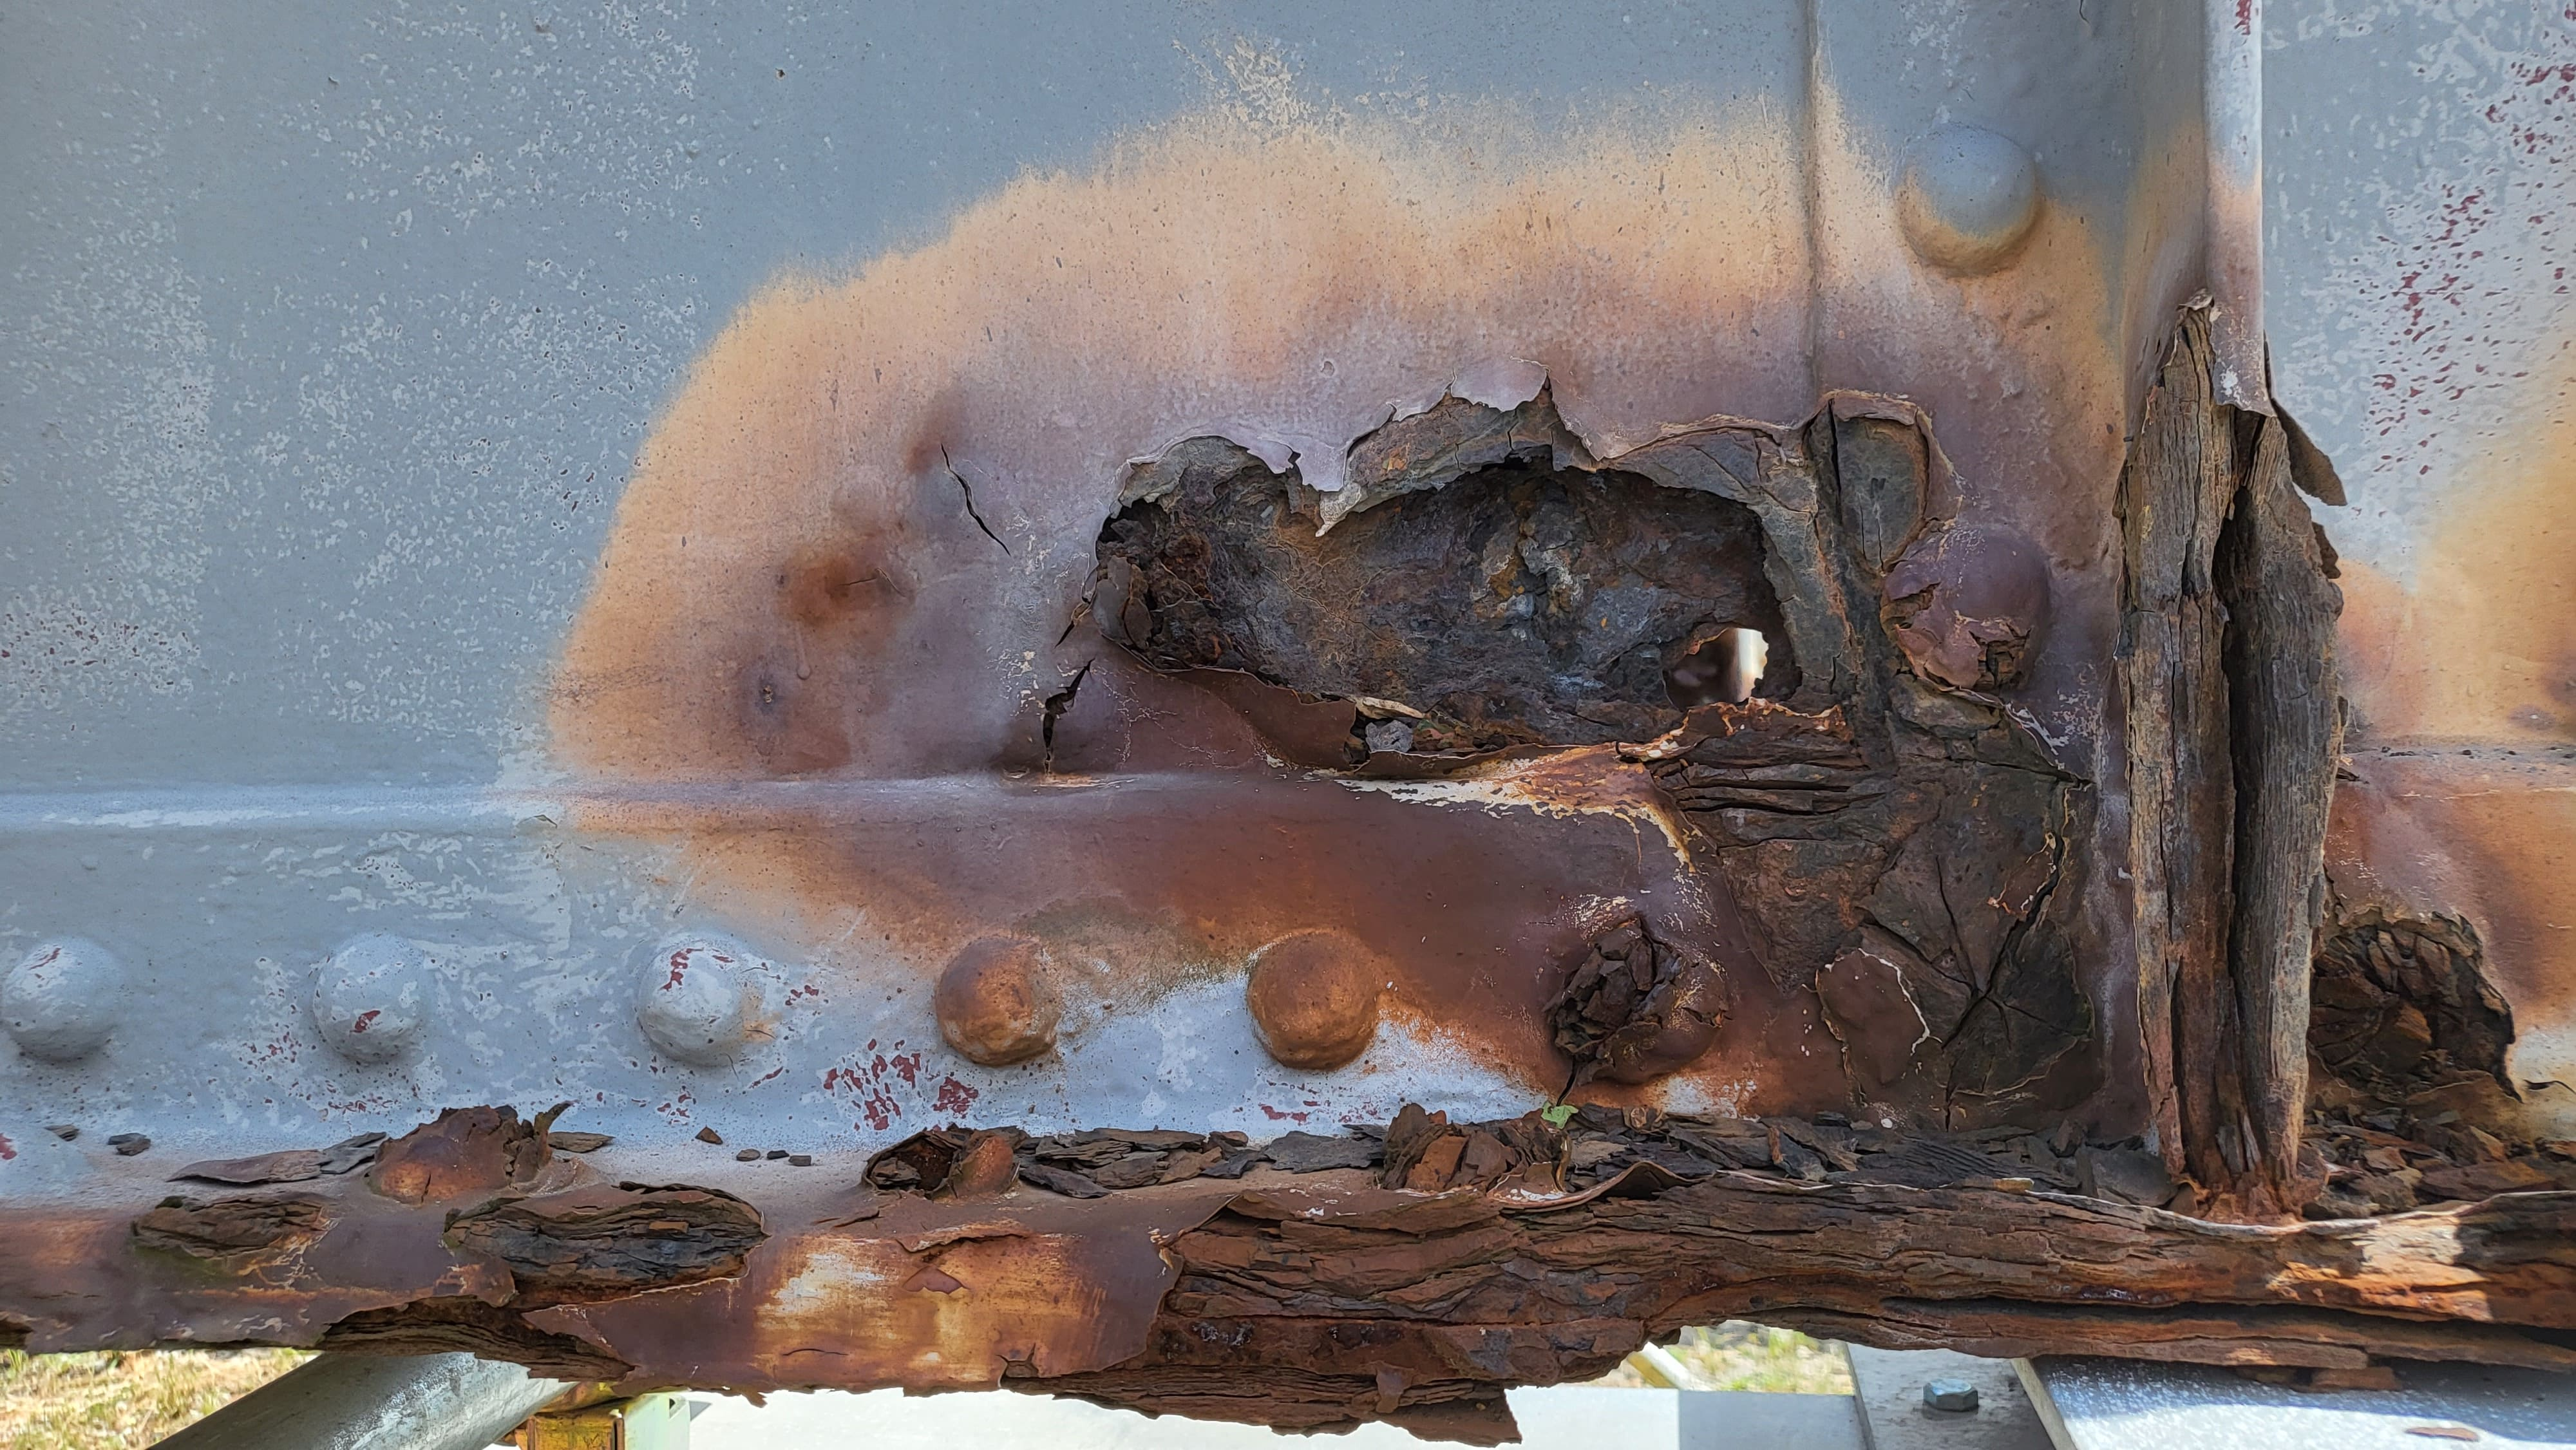
\includegraphics[width=\textwidth]{imgs/ch2/rivet-cor-1.jpg}%rivet-cor.png
        \caption{Corrosion of rivet}
        \label{fig-corriv}
    \end{subfigure}
    
    \begin{subfigure}[t]{0.85\linewidth}
        \centering
        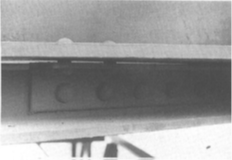
\includegraphics[width=\textwidth]{imgs/ch2/rivet-loss.png}
        \caption{Loosing of rivet}
        \label{fig-losriv}
    \end{subfigure}
    \caption{Aging condition of rivet}
\end{figure}


\begin{figure}
    \centering
    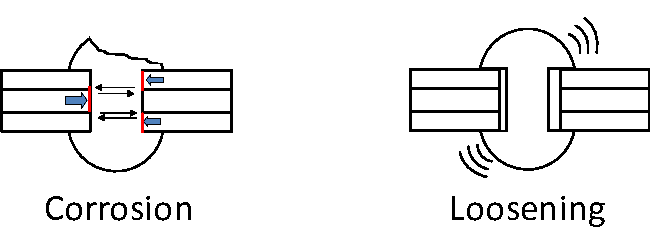
\includegraphics[width=0.8\textwidth]{imgs/ch2/rivet-issue.pdf}
    \caption{corrosion and loosing of aging rivet}
    \label{fig-rivetisu}
\end{figure}

\subsection{Mechanical behavior of riveted joint}

There are three types of resistance present in a riveted joint: friction, bearing, and shear. When it comes to force transfer utilizing a single rivet, there are two types: single-lap and double-lap as shown in Fig.\ref{fig-lapconnec}. Although an increase in the number of plates results in multi-sided shear, these two types are the fundamental structures of riveted joints in terms of force action. The forces transferred by the rivet only take into account the forces perpendicular to the rivet axis, such as direct tensile force. They do not consider the impact of axial tensile forces on the rivet head or its design. When two plates are joined by riveting, frictional forces transmit the load and restrict plate movement. This enhances the joint's strength, although it is not considered during the design process. Fig.\ref{fig-rsdisri} illustrates that the stress distribution, encompassing the rivet and the plate, is highly intricate. However, for practical purposes, it can be simplified into the following three types to facilitate design calculation for engineering.


\subsection{Literature review}

Research has shown that riveted connections have been extensively studied in various countries in the past. However, most of the research has focused on the study of sound riveted connections, while studies on the deterioration of connections over time have evaluated the relationship between the structural integrity of the riveted structure and the service life, and have reported on the occurrence of damage and component performance degradation. The residual carrying capacity of corroded riveted beams and the estimation formulas for their carrying capacity have been specifically assessed through experiments and finite element analysis. However, these studies primarily focus on the residual carrying capacity of riveted connections and the residual performance of materials. There is less research on the repair and strengthening methods of riveted bridges, especially when rivets are replaced by high-strength bolts due to corrosion, and the changes in joint performance and load transfer mechanisms are not yet well understood.

\begin{figure}
    \centering
    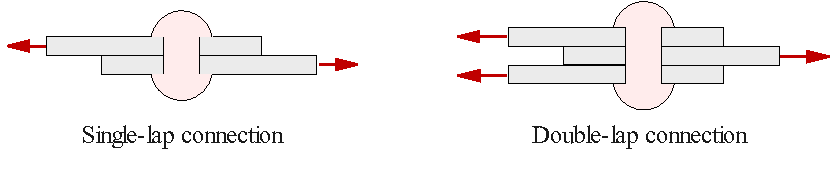
\includegraphics[width=0.85\textwidth]{imgs/ch2/lap-connec.pdf}
    \caption{Single \& Double lap connection}
    \label{fig-lapconnec}
\end{figure}


\begin{figure}
    \centering
    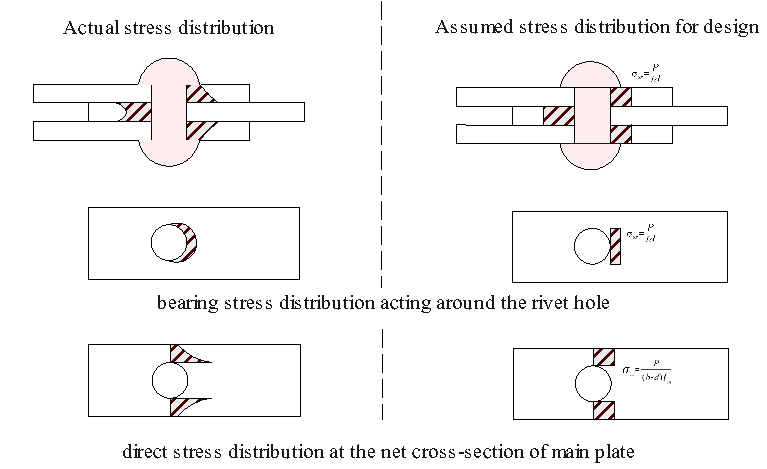
\includegraphics[width=0.85\textwidth]{imgs/ch2/bstressdistr-0.pdf}
    \caption{Stress distribution of double-lap riveted connection}
    \label{fig-rsdisri}
\end{figure}


\subsubsection{Assessment of riveted bridge: fatigue, strength, corrosion}
Extensive research on riveted joints has been conducted in numerous countries in the past. However, the majority of these studies focused on the examination of intact riveted joints. Haghani et al.\cite{haghani2012} conducted a comprehensive review of fatigue damage cases in over 100 bridges. Hołowaty et al. \cite{holowaty2022} examined the structural condition of 13 aged steel bridges constructed between 1873 and 1890, as well as 17 bridges spanning from 1907 to 1983.
Bacinskas et al. \cite{BACINSKAS2013136} conducted a study on the structural condition and behavior of a riveted steel truss bridge using full-scale static and dynamic testing. Aktan et al. \cite{aktan1994destructive} conducted a comprehensive series of nondestructive and destructive tests on two 80-year-old steel truss bridges that had been decommissioned, and the results show that, after completing each destructive test, no evidence of distortion or failure was found in the retrofitted connections. The effectiveness of the retrofit was demonstrated under the heavy concentrated loads experienced during destructive testing. Consequently, it can be deduced that similar bridges can be retrofitted to acceptable levels of safety with minimal effort and cost. Wang et al. \cite{wang2012} conducted a series of tests on an original steel angle obtained from a riveted truss Lanzhou Zhongshan Bridge, which was constructed in 1909. These tests examined the material mechanics, fracture behavior, and fatigue properties of the angle. Kossakowski \cite{kossakowski2013fatigue} presented the research findings on the fatigue strength of steel extracted from a railway bridge that had been in service for over a hundred years. The study focuses on analyzing and investigating the corrosion rate and assessing steel degradation. Małgorzata \cite{Skorupa2015InvestigationJoint} conducted experiments to investigate the load transfer mechanism of single-lap riveted joints and proposed a straightforward model to explain the transfer process. Gocál and Odrobiňák \cite{Gocal2020OnBridges} examines the influence of atmospheric corrosion on the load-carrying capacity of old riveted bridge structures. It analyzes the results and discusses the importance of long-term in situ corrosion measurements, as well as regular inspections for existing bridges. Reichle \cite{Reichle1999} analyzes the behavior of corroded rivets used in the connections of structural steel members. In particular, the material loss caused by corrosion is quantified using finite element analysis. And the findings of a parametric study and offers recommendations for deciding when to replace corroded rivets were presented. Zice \cite{Zice2023} conducted to investigate influences of the corrosion extent of rivet heads with artificial corrosion damage on the mechanical behaviour.

Numerous studies\cite{imam2008,Ryoichi2013,1987163,hisanori1991} have assessed the structural integrity of aging riveted connections in relation to their service life, and have reported on the correlation between the rate of damage and the decline in member performance. Through experiments and FEM analyzes\cite{nakata2016, Yurika2019,chen2022jp,cheniabse2022,Pipinato2014ResidualApproach,Bertolesi2021FatigueApproach}, the assessment of the remaining load bearing capacity of corroded riveted girders and the development of formulas for estimating said capacity have also been clarified. 

\subsubsection{Repair and reinforcement}
Lima et al.\cite{lima2008} presented the rehabilitation process of a century-old steel truss bridge with riveted connections in Canada. Kääriäinen \& Pulkkinen \cite{kaaria2002} documented the rehabilitation of the Tornionjoki steel truss bridge. Kimura et al.\cite{kimura2009} performed static loading tests to evaluate the strength of corroded rivet parts as well as the replaced parts using high-strength bolts. These components were obtained from a steel railway bridge that had been decommissioned, as well as from highway bridges. Siwowski \cite{siwowski2013} documented the rehabilitation of a continuous Warren-type steel truss bridge consisting of five spans, constructed in 1961. Gheitasi et al. \cite{Gheitasi2022} documented the rehabilitation of a historic steel truss bridge, which was 133 years old. The rehabilitation process involved partial dismantling, temporary relocation, and retrofitting, with a focus on various aspects of design and construction. Heydarinouri et al. \cite{Heydarinouri2021} presented a retrofit system that utilized pre-stressed CFRP bars to strengthen the double-angle connections between the stringers and floor beams of a riveted railway bridge in Switzerland, which had been in service for 92 years.

\subsection{Clamping force (Preload) of rivet}

When the heated rivet cools and hardens, the shrinkage of the rivet shaft introduces a significantly higher clamping force. In the past, there have been few studies to assess the clamping force of rivets due to limitations in measurement techniques. In the past, it was believed that the rivet would provide a clamping force equivalent to the yield point of the steel \cite{VanMaarschalkerwaart1982FatigueJoints}. However, subsequent experiments have shown that a clamping force of the yield point of the shaft part can be achieved by incorporating a relatively long rivet shaft ($>100 mm$). In contrast, when a short rivet shaft is present, the mean value of the clamping force introduced is lower, and the dispersion is also higher \cite{Zhou1994FatigueMembers, Baron1953TheJoints}. The deviation of the rivet head is believed to have a significant impact on the clamping force for short rivet axes.

Previous research findings \cite{Zhou1994FatigueMembers} indicate that the clamping force is dependent on the steel grade, particularly for rivets with a diameter of 24.5 mm. Therefore, Åkesson \cite{Akesson2010} refers to the nominal tensile stress caused by the clamping force in the axial section of the rivet as the clamping stress. The clamping stress to yield stress ratio of the rivet material was a crucial parameter in assessing the rivet clamping force. The average ratios were 0.61 and 0.77 for the rivet shaft lengths of 75 mm and 125 mm respectively. K{\"u}hn \cite{Kuhn2008AssessmentLife} have shown that the tightening force of st52 material rivets is lower than that of st37 material rivets. Heinemeyer \cite{Heinemeyer2011TheConnections} presents recent investigations on the impact of rivet head corrosion on the pre-stressing of the rivet, achieved through milling the rivet's head and conducting numerical simulations. It also presents fatigue tests that provide initial results for assessing the remaining lifespan of a riveted connection with reduced rivet stress.

The above mentioned previous studies mainly conducted tests in laboratory settings utilizing relatively long rivet shafts. Nevertheless, the actual clamping force introduced during riveting real bridges, particularly in-situ, differs to some extent from these experimental findings due to mistakes made during the riveting operation. A previous study8) removed rivets from real bridge girders and flanges to measure the residual rivet clamping force. Akesson \cite{Akesson2010} and Baron \& Larsson \cite{Baron1953TheJoints} reported comparable outcomes. Both sets of experimental data indicated that the length of the rivet shaft had a significant impact on the clamping force. Fig.\ref{fig-preload-rivet}  showed that a relatively long rivet shaft increased the average clamping force while decreasing its variance. Moreover, Leonetti \cite{Leonetti2020RivetBridges} also found that the number of plates also had an influence on the clamping force of the rivet. The misalignment of the holes of the plates has been reported to be caused by construction errors.

\begin{figure}
    \centering
    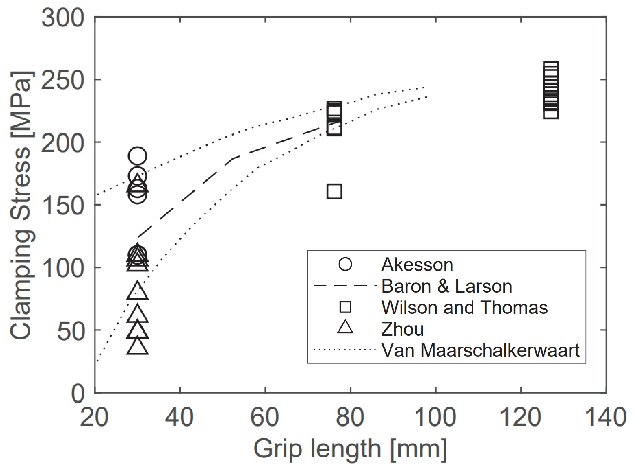
\includegraphics[width=0.8\textwidth]{imgs/ch2/preload-rivet.pdf}
    \caption[The variability of the clamping stress as a function of the grip length for carbon steels.]{The variability of the clamping stress as a function of the grip length for carbon steels. (figure cite from \cite{Leonetti2020RivetBridges}, experimental data from Åkesson \cite{Akesson2010},Wilson and Thomas \cite{Wilson1938FatigueJoints}, and Zhou \cite{Zhou1994FatigueMembers}. Also the average trend from Baron \& Larson \cite{Baron1953TheJoints}, and upper and lower bounds from van Maarschalkerwaart \cite{VanMaarschalkerwaart1982FatigueJoints} are reported.)}
    \label{fig-preload-rivet}
\end{figure}


\subsection{Remaining issue}
However, the primary focus of these studies is on the residual carrying capacity of riveted connections and the residual performance of materials. Insufficient research has been conducted on the repair and strengthening methods of riveted bridges, especially in cases where corrosion leads to the substitution of rivets with high-strength bolts, resulting in limited understanding of the alterations in joint performance and load transfer mechanisms. Steel riveted bridges hold significant cultural and historical value as a part of our constructive heritage from the previous century. Numerous iron and steel riveted bridges are of historical importance, requiring restoration and preservation, and are currently operational.

\section{Friction type bolted connection}

\subsection{Background}

Friction-type High-strength bolt connections have been widely used in building steel structures recently due to their ease of installation, higher bearing capacity, and superior anti-fatigue performance. The high-strength bolt connection can be classified into bearing type and friction type based on the difference in force transmission patterns as shown in \ref{fig-fricandbearing}. In the case of the bearing type, the connection's bearing capacity depends on the resistance of the hole wall and the shear resistance of the bolts. In the case of the friction type, the force is transmitted through friction between the faying surfaces of the plates. The resistance of the bearing type connection is typically higher than that of the friction type. However, the bearing type connection is not directly suitable for fatigue and dynamic loads.

\begin{figure}
    \centering
    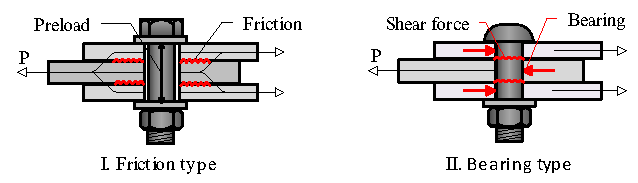
\includegraphics[width=0.85\textwidth]{imgs/ch2/fricandbearing.pdf}
    \caption{Schematic of load transmit mechanism of friction-type and bearing-type bolted connection}
    \label{fig-fricandbearing}
\end{figure}

The mechanical properties of bolted joints have a direct impact on their load-bearing capacity. The spacing, strength, and stress state of bolts all play a crucial role in determining the mechanical properties of high-strength bolted joints. Extensive research has been conducted over the years to investigate the various factors that affect these properties \cite{peng2015,Lyu2019NumericalSteels,Brian1996EdgeOcnnections,wang2020interface,hirashima2004experimental}. This research has helped identify ways to optimize the performance of bolted joints, ensuring the safety and longevity of structures in diverse applications. Understanding the factors that influence these properties enables engineers and designers to make informed decisions regarding material selection and structural design to meet specific performance requirements.

The construction of new bridges often entails several design challenges. Among these challenges is the requirement to enhance the strength of bridge components to withstand increased external live loads, without necessitating a larger overall structure. This necessity for adjustments has gained prominence in recent years, coinciding with the growing utilization of high-strength steels in bridge construction.

To fulfill this requirement, the bolted joints within the steel bridge structure must be engineered to endure the augmented strength of the steel components. However, the strength of friction-type joints is influenced by two primary factors: the quantity of bolts employed and the slip coefficient. 

Increasing the number of bolts is a simple and effective measure. However, an increase in the number of bolts means that the size of the joint will become larger, resulting in added weight. Large joints bring about several disadvantages, such as decreased load-carrying capacity with increasing side length of the joint. Additionally, an increase in the number of bolts complicates the management and maintenance of the bolt group, thereby increasing the maintenance costs of the bridge.

\subsection{Technical Problem} %%todo , add the long bolted joint figure.
Problems arise when utilizing long or large friction-type bolted joints as the joint length increases. Firstly, these excessively long bolted joints can cause interference with secondary members, such as stiffeners and diaphragms, located in close proximity to the joint. Therefore, it becomes necessary to reduce the joint length while maintaining the design strength. Typically, a friction-type bolted joint combined with a weld is employed to meet the design strength requirements of a joint. Previous studies have demonstrated the reliability and feasibility of friction-type bolted joints combined with welds \cite{solodov2021,Thomas2000,Chang2019361,KHANDEL2022107036}. Combinations of welded-bolted connections are sometimes utilized in steel structures to improve their strength. However, However, this combination methods is inefficient in terms of load bearing capacity enhancement, also the certain environments, such as those with limited space or requiring work at height, are not conducive to onsite welding during bridge construction. Additionally, welding destroys the original coating of steel parts, necessitating reapplication of the protective paint to the joints. Consequently, the construction of combined welded-bolted connections for steel bridge joints that require onsite joining becomes highly challenging. Thus, suitable approaches are required to reduce the length of bolted joints without compromising their strength.

Second, as the length of the joint (defined as the spacing between the first and last fasteners in a joint) increases, the resistance that can bolt provide decreases to a value lower than the slip strength because the distribution of the bolts inside the joint becomes uneven. As the joint length increases with an increasing number of bolts in a line, the differential deformations in the main plate causes shear failure at the end bolts before all bolts can develop their full shearing strength. This "unbuttoning" phenomenon has been observed for all types of fasteners including rivets \cite{fisher1965behavior}. Bendigo et al.\cite{bendigo1963long} concluded that for longer connections, end bolts are sheared before all the bolts can develop their full shear strength. For short connections, the average shear stress is approximately 85\% that of a single bolt; however, for a 52.5 inch long connection, bolts only develop 60\% of their strength. Kamei et al. \cite{KAMEI2000} also showed that the serviceability limit strength decreases by approximately 2.5 $\%$ for each additional row.  Tan et al.\cite{Tan2022} considered that when the number of rows of bolts is more than 5, the force transmission ratio of the end bolt is 0.389.

Owing to the above issues, specifications for long-bolted joints, such as AASHTO \cite{AASHTO2020}, Eurocode3 \cite{eurocode3}, as well as Japanese and Chinese, all provide a reduction factor based on the length of the bolted joint \cite{eccs1985,isohtb,douji2017}. Furthermore, owing to uneven load sharing, the bolts cannot simultaneously fracture, and the ultimate limit bearing capacity decreases \cite{Takai2021BoltUnbuttoning,Peng2013FeaDimensions,peng2010,longstainless2022}. 

Considering the installation space requirements and strength problems associated with long-bolted joints, a rational compact joint must be developed to allow the use of fewer bolts to transmit more load, which could also improve the service limit capacity of the joints.

\section{Bearing type bolted connection}

\subsection{Background}

The HSB bearing type connection is a connection method based on the idea that, as in the case of friction connections, a preload is usually introduced into the bolt and frictional resistance is used for normal loads, while shear resistance of the bolt shaft and bearing resistance of the base metal and the connecting plate are expected for emergency loads, such as an earthquake \cite{rivet1977}. There are four types of bolt that can be used for support connections: those with a shape similar to that of a friction connection, those with an interference fit (hammered-in type), and the resin-injected bolt or the mechanical bolt-rivet. These bolts are characterised by their method of load transmission, relying primarily on bearing against the sides of holes in the fasteners and friction to transmit forces in a hybrid manner.

Bearing bolts operate on a simple mechanical principle: When a load is applied to the connected structure, it induces direct bearing forces on the bolt shank. These forces, in turn, are transferred to the material surrounding the bolt holes by bearing stress. These bolts are not designed to be preloaded; they operate as soon as the load causes the connected elements to press against the bolt. For optimum performance, the hole diameter is made slightly larger than the diameter of the bolt for ease of installation; however, this clearance must be minimal to maintain load transfer without yielding or excessive deformation. ASTM standards \cite{ASTM-bolt} and others provide guidelines for these tolerances to ensure proper function.

In recent years, the use of bearing type connections has been reported\cite{morikawa2002} in cases where the required performance of the friction faying surface is not satisfied, such as in the case of a reinforce method for fatigue cracks at the corner of steel piers, but the number of applications to actual bridge main members is extremely small. 

Although the bearing-type connection can offer much higher strength compared to the friction-type connection \cite{Li2020bbolt,perry1981bearing,kim1999bearing}, it also faces a series of issues such as poor construction performance and high precision requirements, their application comes with inherent challenges. First, the precise required tolerances between the bolts and the holes. Since load transfer depends on the bearing of the bolt against the edge of the hole, any significant misalignment or incorrect size can lead to reduced load capacity or even structural failure. Furthermore, these connections are susceptible to slipping when exposed to dynamic or cyclic loads, necessitating careful consideration of the slip coefficients of the connected materials and the potential for fatigue.

Moreover, in environments prone to corrosion or where long-term durability is a concern, protective measures must be implemented to preserve the integrity of the bearing-type bolts. Regular inspections are vital to detect any signs of wear, corrosion, or loosening that could compromise the connection's integrity.

In summary, it can be expected that in the future bearing type bolts will be a fundamental element in the design of steel structures, offering a balance between strength, ease of assembly and cost effectiveness.

\subsection{Interference fit bolt}

In Japan, a specialized high-strength bolt bearing type inteference fit bolt (\ac{IFHSB}) is present, as shown in Fig. \ref{fig-onebbolt}. 
%todo! 轴部有rib一般要求大于孔径,balabala,等要求

Bearing-type bolts are widely employed for connecting steel bridge piers, owing to their substantial load-bearing capacity, which can accommodate large-scale earthquakes \cite{Guo20205}. Moreover, they can reduce the fatigue present in bolt holes, thereby increasing their fatigue strength. However, the stringent requirements for bolt-hole accuracy during the installation of bearing-type bolts make their use uncommon in other parts of the bridge.



\begin{figure}
    \centering
    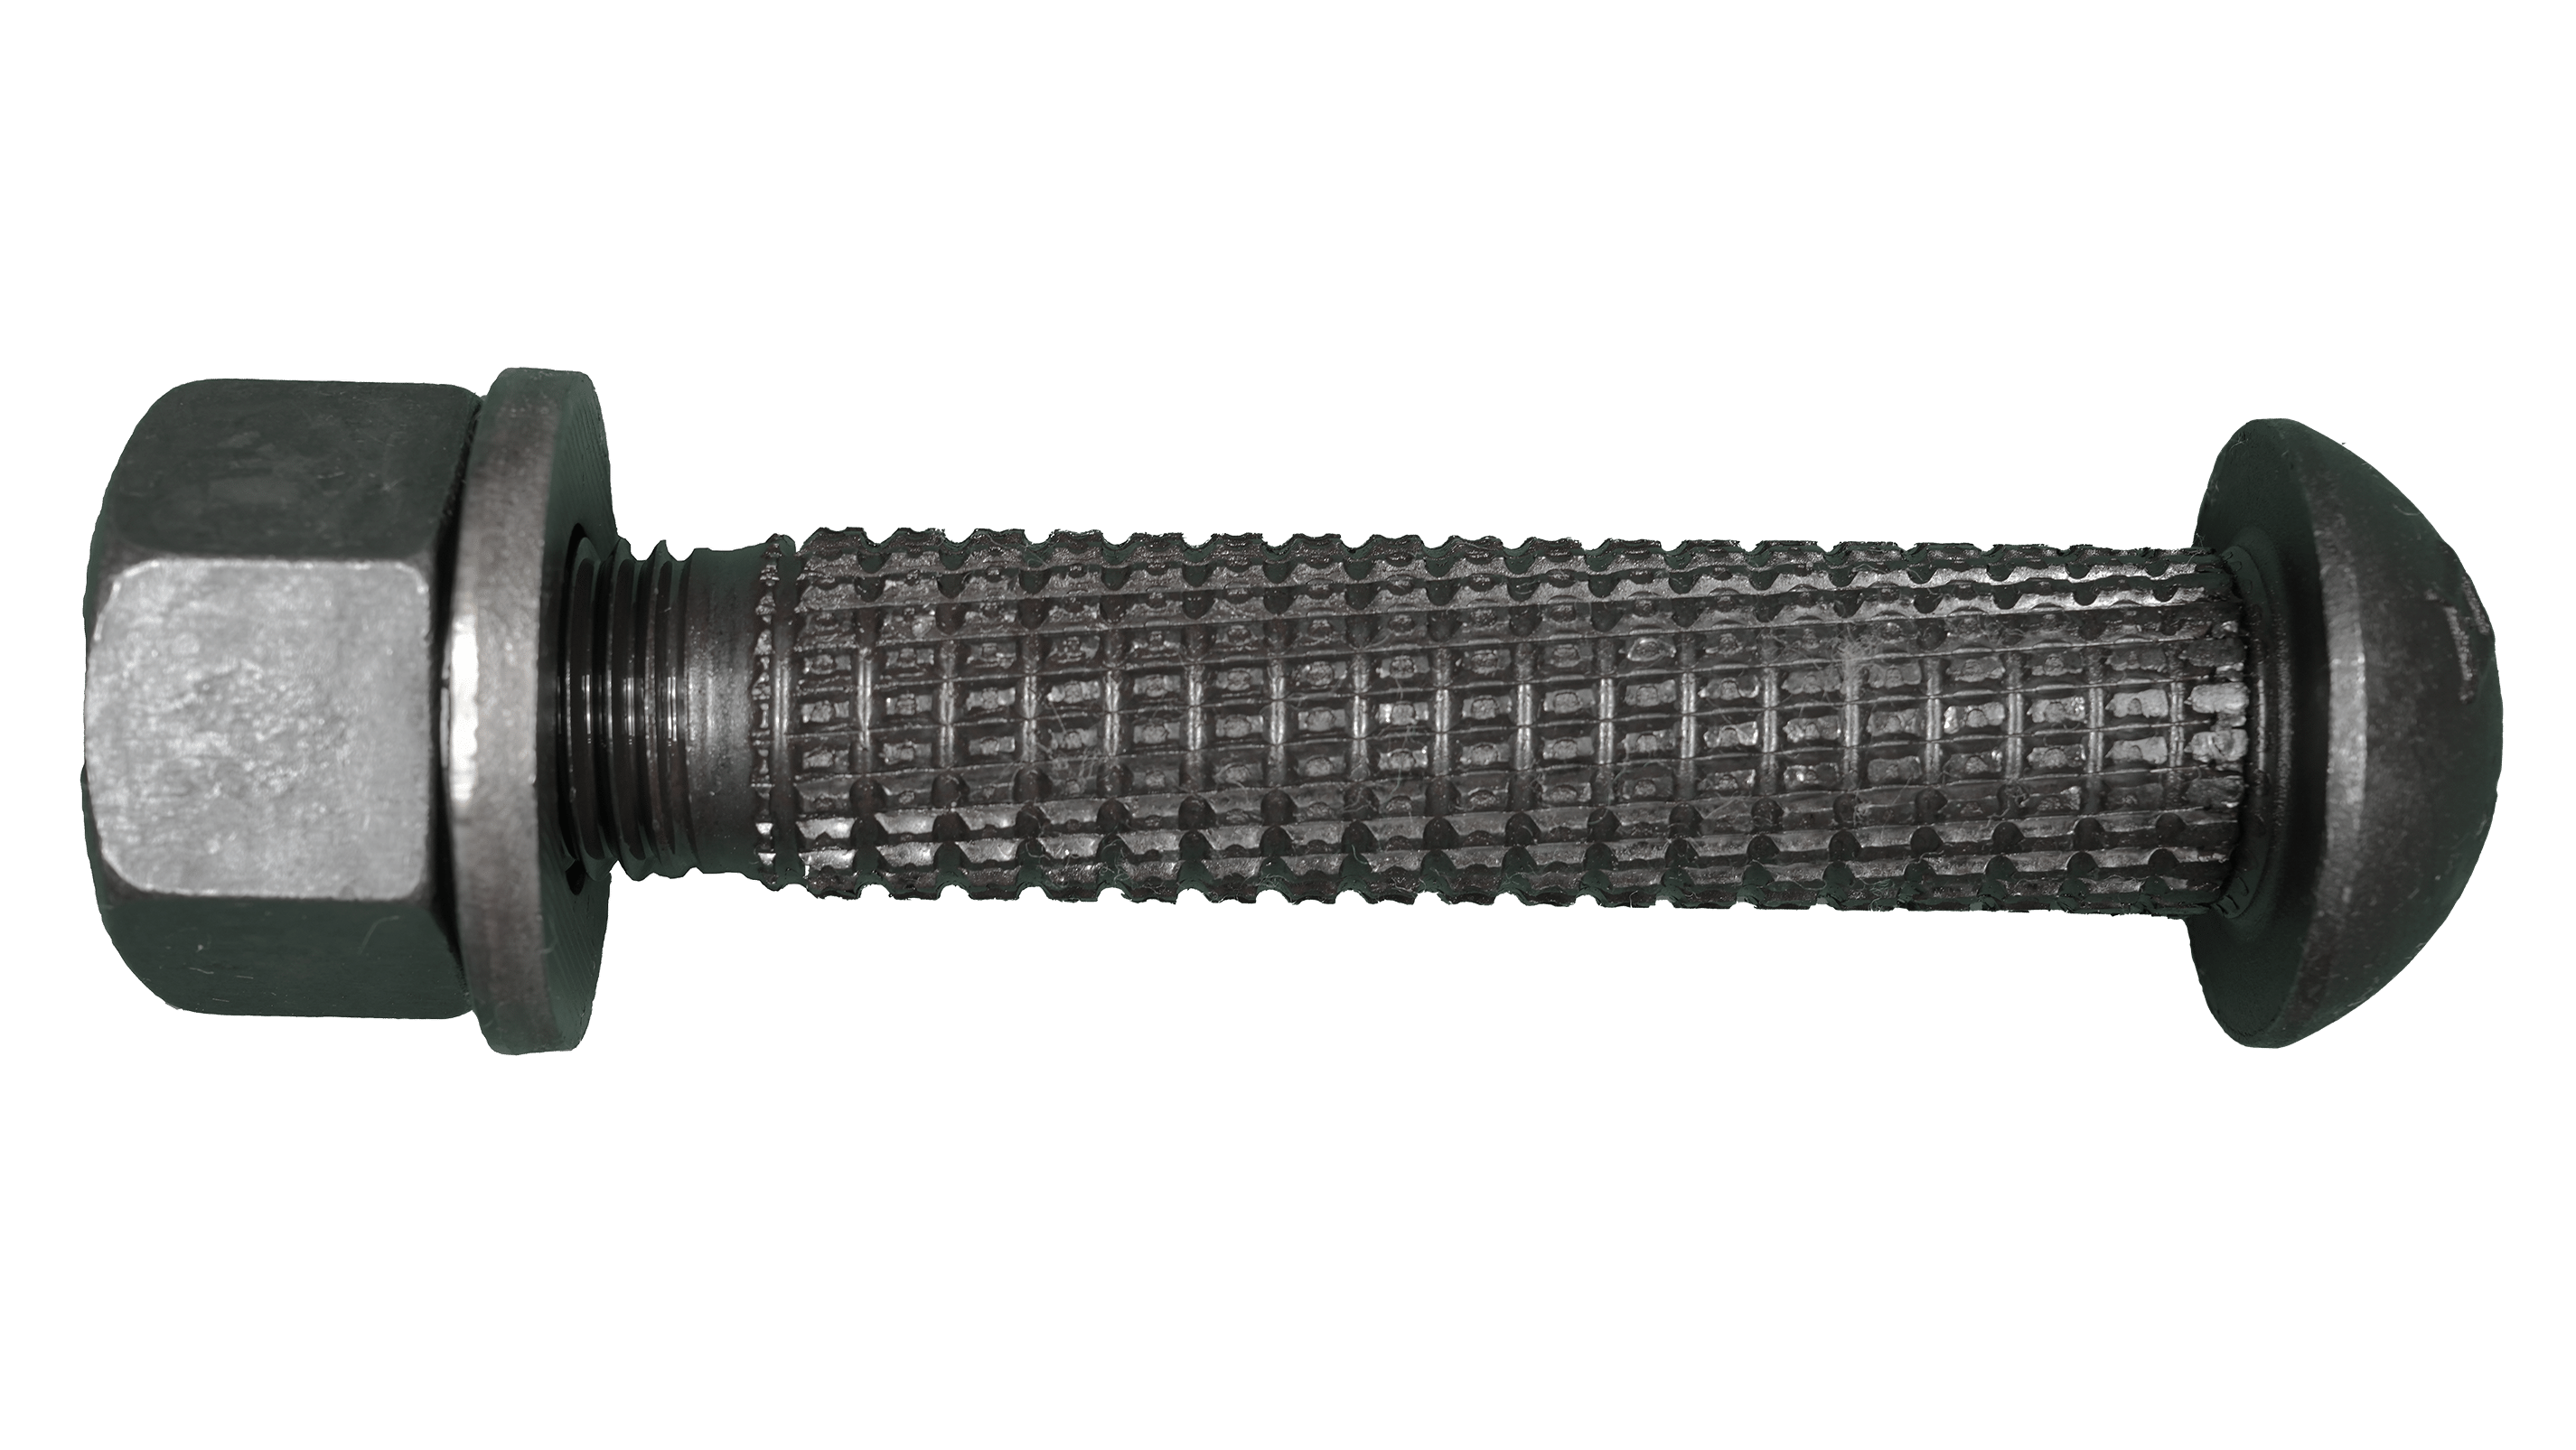
\includegraphics[width=0.8\linewidth]{imgs/ch2/oneBbolt.png}
    \caption{Bearing-type Inteference fit bolt (M22, Diameter = 23.5mm), Made in Kobelco Bolt, Ltd.}
    \label{fig-onebbolt}
\end{figure}

\begin{figure}
    \centering
    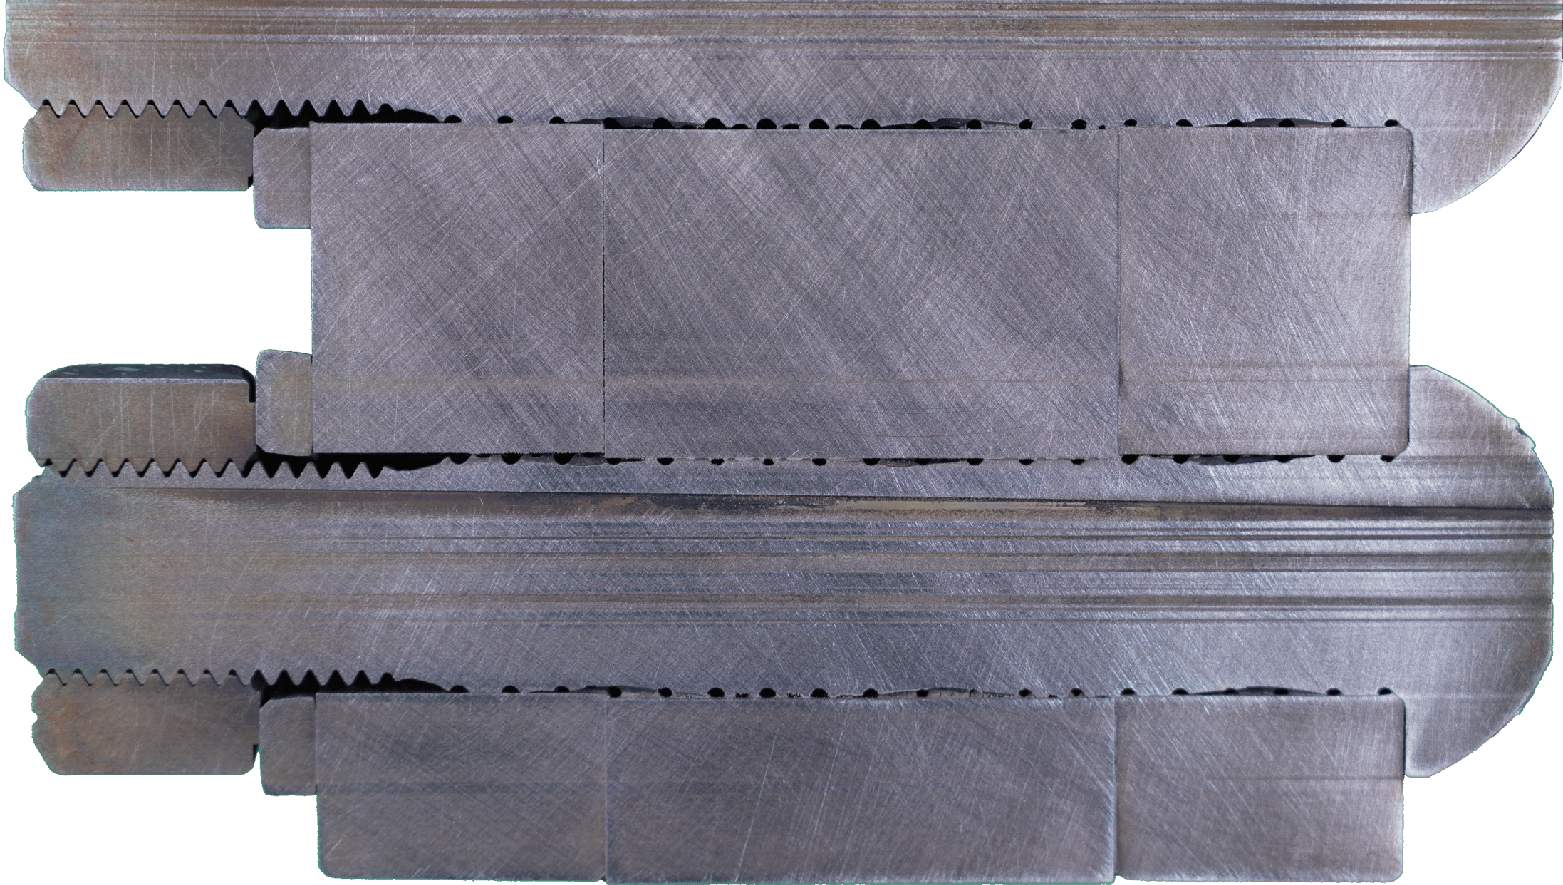
\includegraphics[width=0.8\linewidth]{imgs/ch2/cs-b1.pdf}
    \caption{Sawed-throug cross-section view of interference fit bolt}
    \label{fig-cs-b1}
\end{figure}




\subsection{Resin injected bolt}

Resin-injected bolts are fasteners in which the gap created by the clearance between the bolt and the wall of the hole is filled with a two-component resin as shown in \ref{fig-resinbolt}. They are an effective alternative for bolts fitted with high-strength friction grip bolts in shear connections where slip is not allowed. Injection bolts are a reliable and relatively low-cost option for repairing and improving existing structures \cite{gresnigt1996injbolt}. They are also being used successfully in constructing new structures. The clearance of an injection bolt is filled via a small hole in its head. Once the resin injection is complete and cures completely, the connection becomes slip-resistant. Bearing and shear of the bolt transfer the shear load. In addition, standard structural bolts can be used to fabricate injection bolts. The bolts and washers have been modified to facilitate the injection of resin. The recommendations of ECCS and the Eurocode3 \cite{eurocode3,EN14399}for executing steel structures establish the design and execution regulations for injection bolts.

This particular bolt is utilized and analyzed in Europe \cite{pedrosa2022injbolt-mec,kolstein2017injbolt-mec,pedrosa2020injbolt-fati,pedrosa2021injbolt-fati,gresnigt2000injtbolt-use,ungermann2023injbolt-mec}; however, there is no examination or usage of it in Asia. A small quantity of research exists regarding this bolt type within Japan \cite{fujino2010resbolt,Ryota2018resbolt}.

\begin{figure}
    \centering
    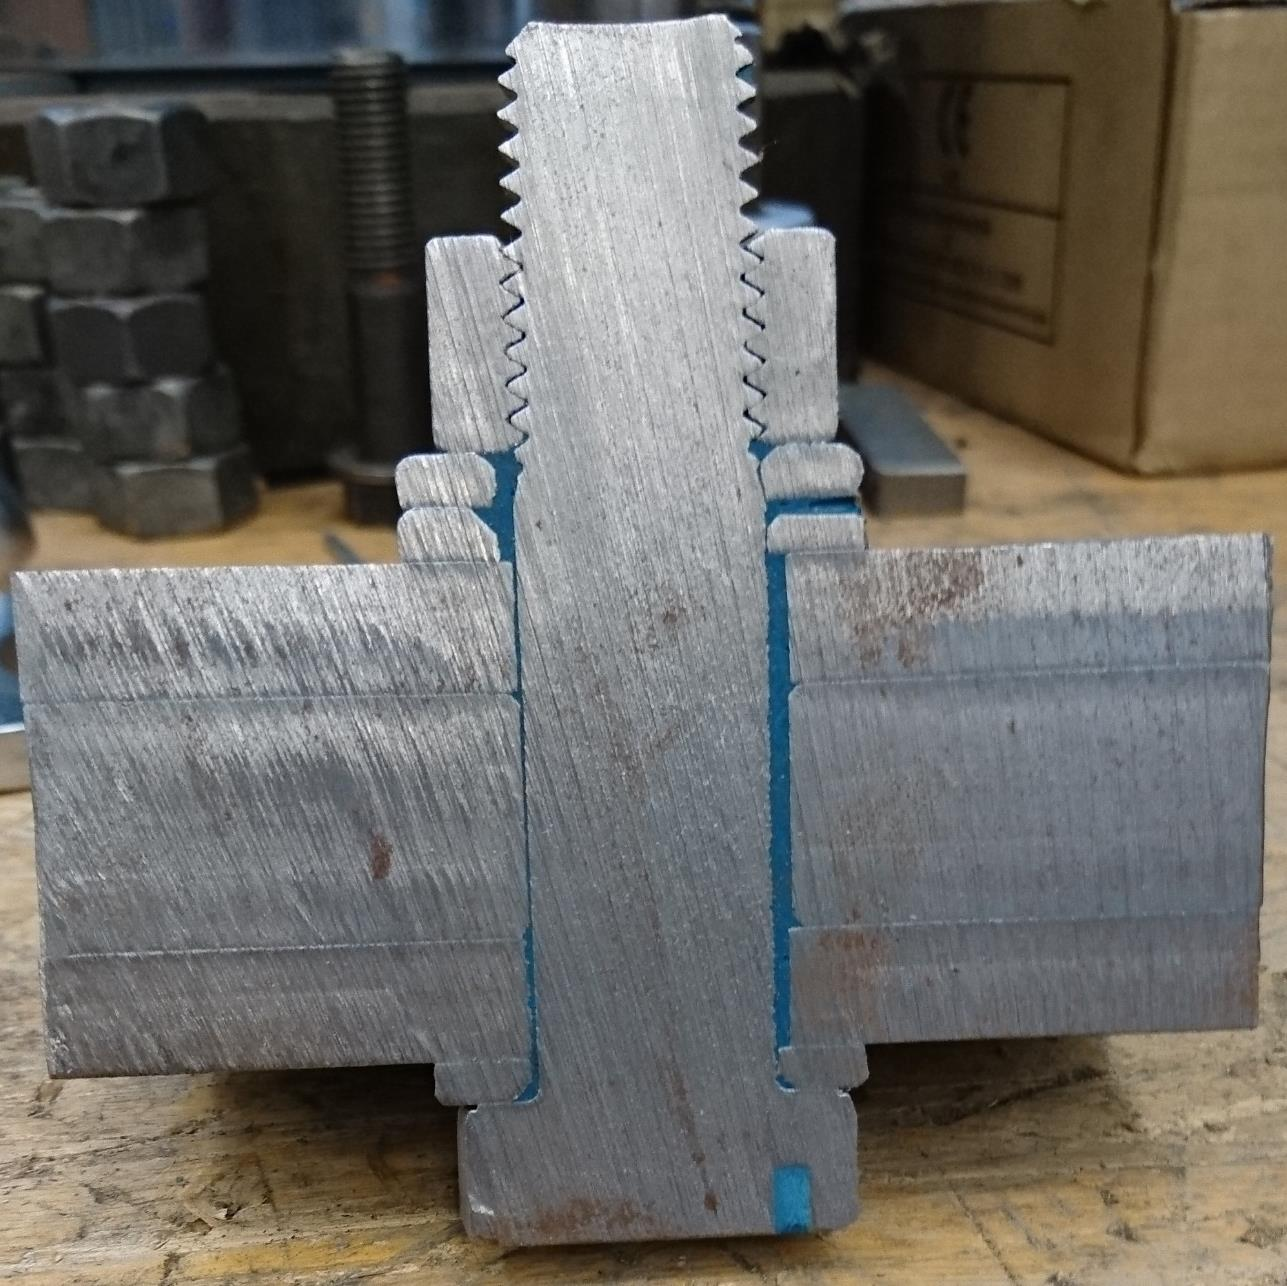
\includegraphics[width=0.85\linewidth]{imgs//ch2/resin-bolt.jpg}
    \caption{Sawed-through (resin) injection bolt connection \cite{Axel2017injbolt}}
    \label{fig-resinbolt}
\end{figure}

\subsection{Other: Mechanical bearing bolt(rivet)}

The above two types of bolted connections have been used in actual steel construction, in addition to these two types of connection, this year Nakamoto et al. (2022) \cite{Nakamoto2022MBBRB} also proposed the mechanical bearing blind bolt (MBBRB), which can be installed on one side and transmits the load through the bearing force between the bolt and the wall of the bolt hole, as well as the friction force on the joint surface as shown in Figure \ref{fig-MBBRB}. The load-displacement relationship of the MBBRB is equivalent to that of the frictional joint using M22F8T up to the slip load. Therefore, the same service limit state can be applied to the MBBRB joint as to the frictional joint.


\begin{figure}
    \centering
    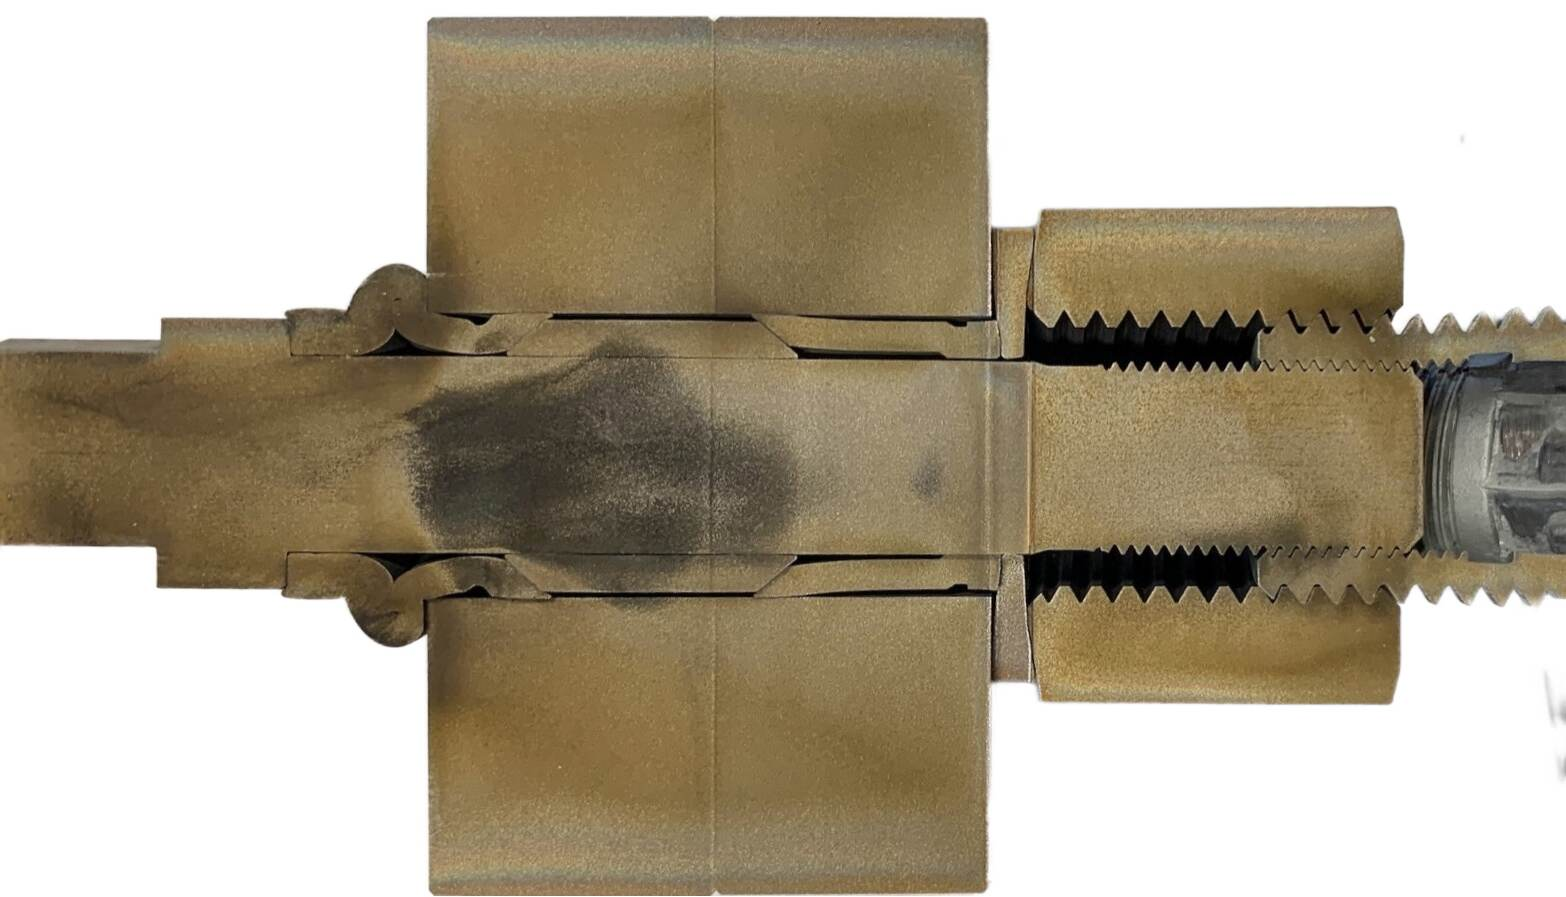
\includegraphics[width=0.85\linewidth]{imgs//ch2/onesidebearingbolt.jpg}
    \caption{Cross-section view of Mechanical Bearing Blind Rivet-Bolts}
    \label{fig-MBBRB}
\end{figure}


\begin{equation}
F_{\mathrm{v}, \mathrm{Rd}}=\frac{\alpha_{\mathrm{v}} f_{\mathrm{ub}} A_{\mathrm{s}}}{\gamma_{\mathrm{M} 2}}
\end{equation}

\section{Hybrid joint}

Joints are usually made of the same type of fastener, however, in some cases two fasteners with different load transmission mechanisms are assembled on the same joint, which is often referred to as a combination joint or hybrid joint as shown in Figure \ref{fig-schehyb}.

The earliest research into hybrid joint was carried out after 1950, when high-strength bolts and welding technology became available. Due to the deterioration of riveted bridges, repair work was carried out on riveted connections, and high-strength bolts with better structural performance became one of the alternatives, but the prevailing view at the time was that connections with different mechanical load transfer mechanisms should not be combined, and, in addition, the prevailing research focused on discussing the performance of high-strength bolts and welds, and therefore research on hybrid joints progressed very slowly.

\begin{figure}[ht]
    \centering
    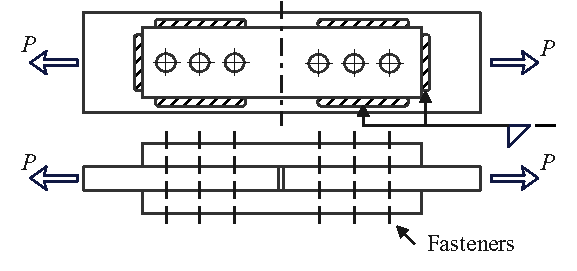
\includegraphics[width=0.75\linewidth]{imgs//ch2/hybrid-sche.pdf}
    \caption{Schematic diagram of Double cover butt hybrid joint}
    \label{fig-schehyb}
\end{figure}

\section{Example of application of hybrid joint}

%高强螺栓和铆钉的混合接头在日本是比较常见的,由于腐蚀铆钉松动等原因


%
\begin{figure}[ht]
    \centering
    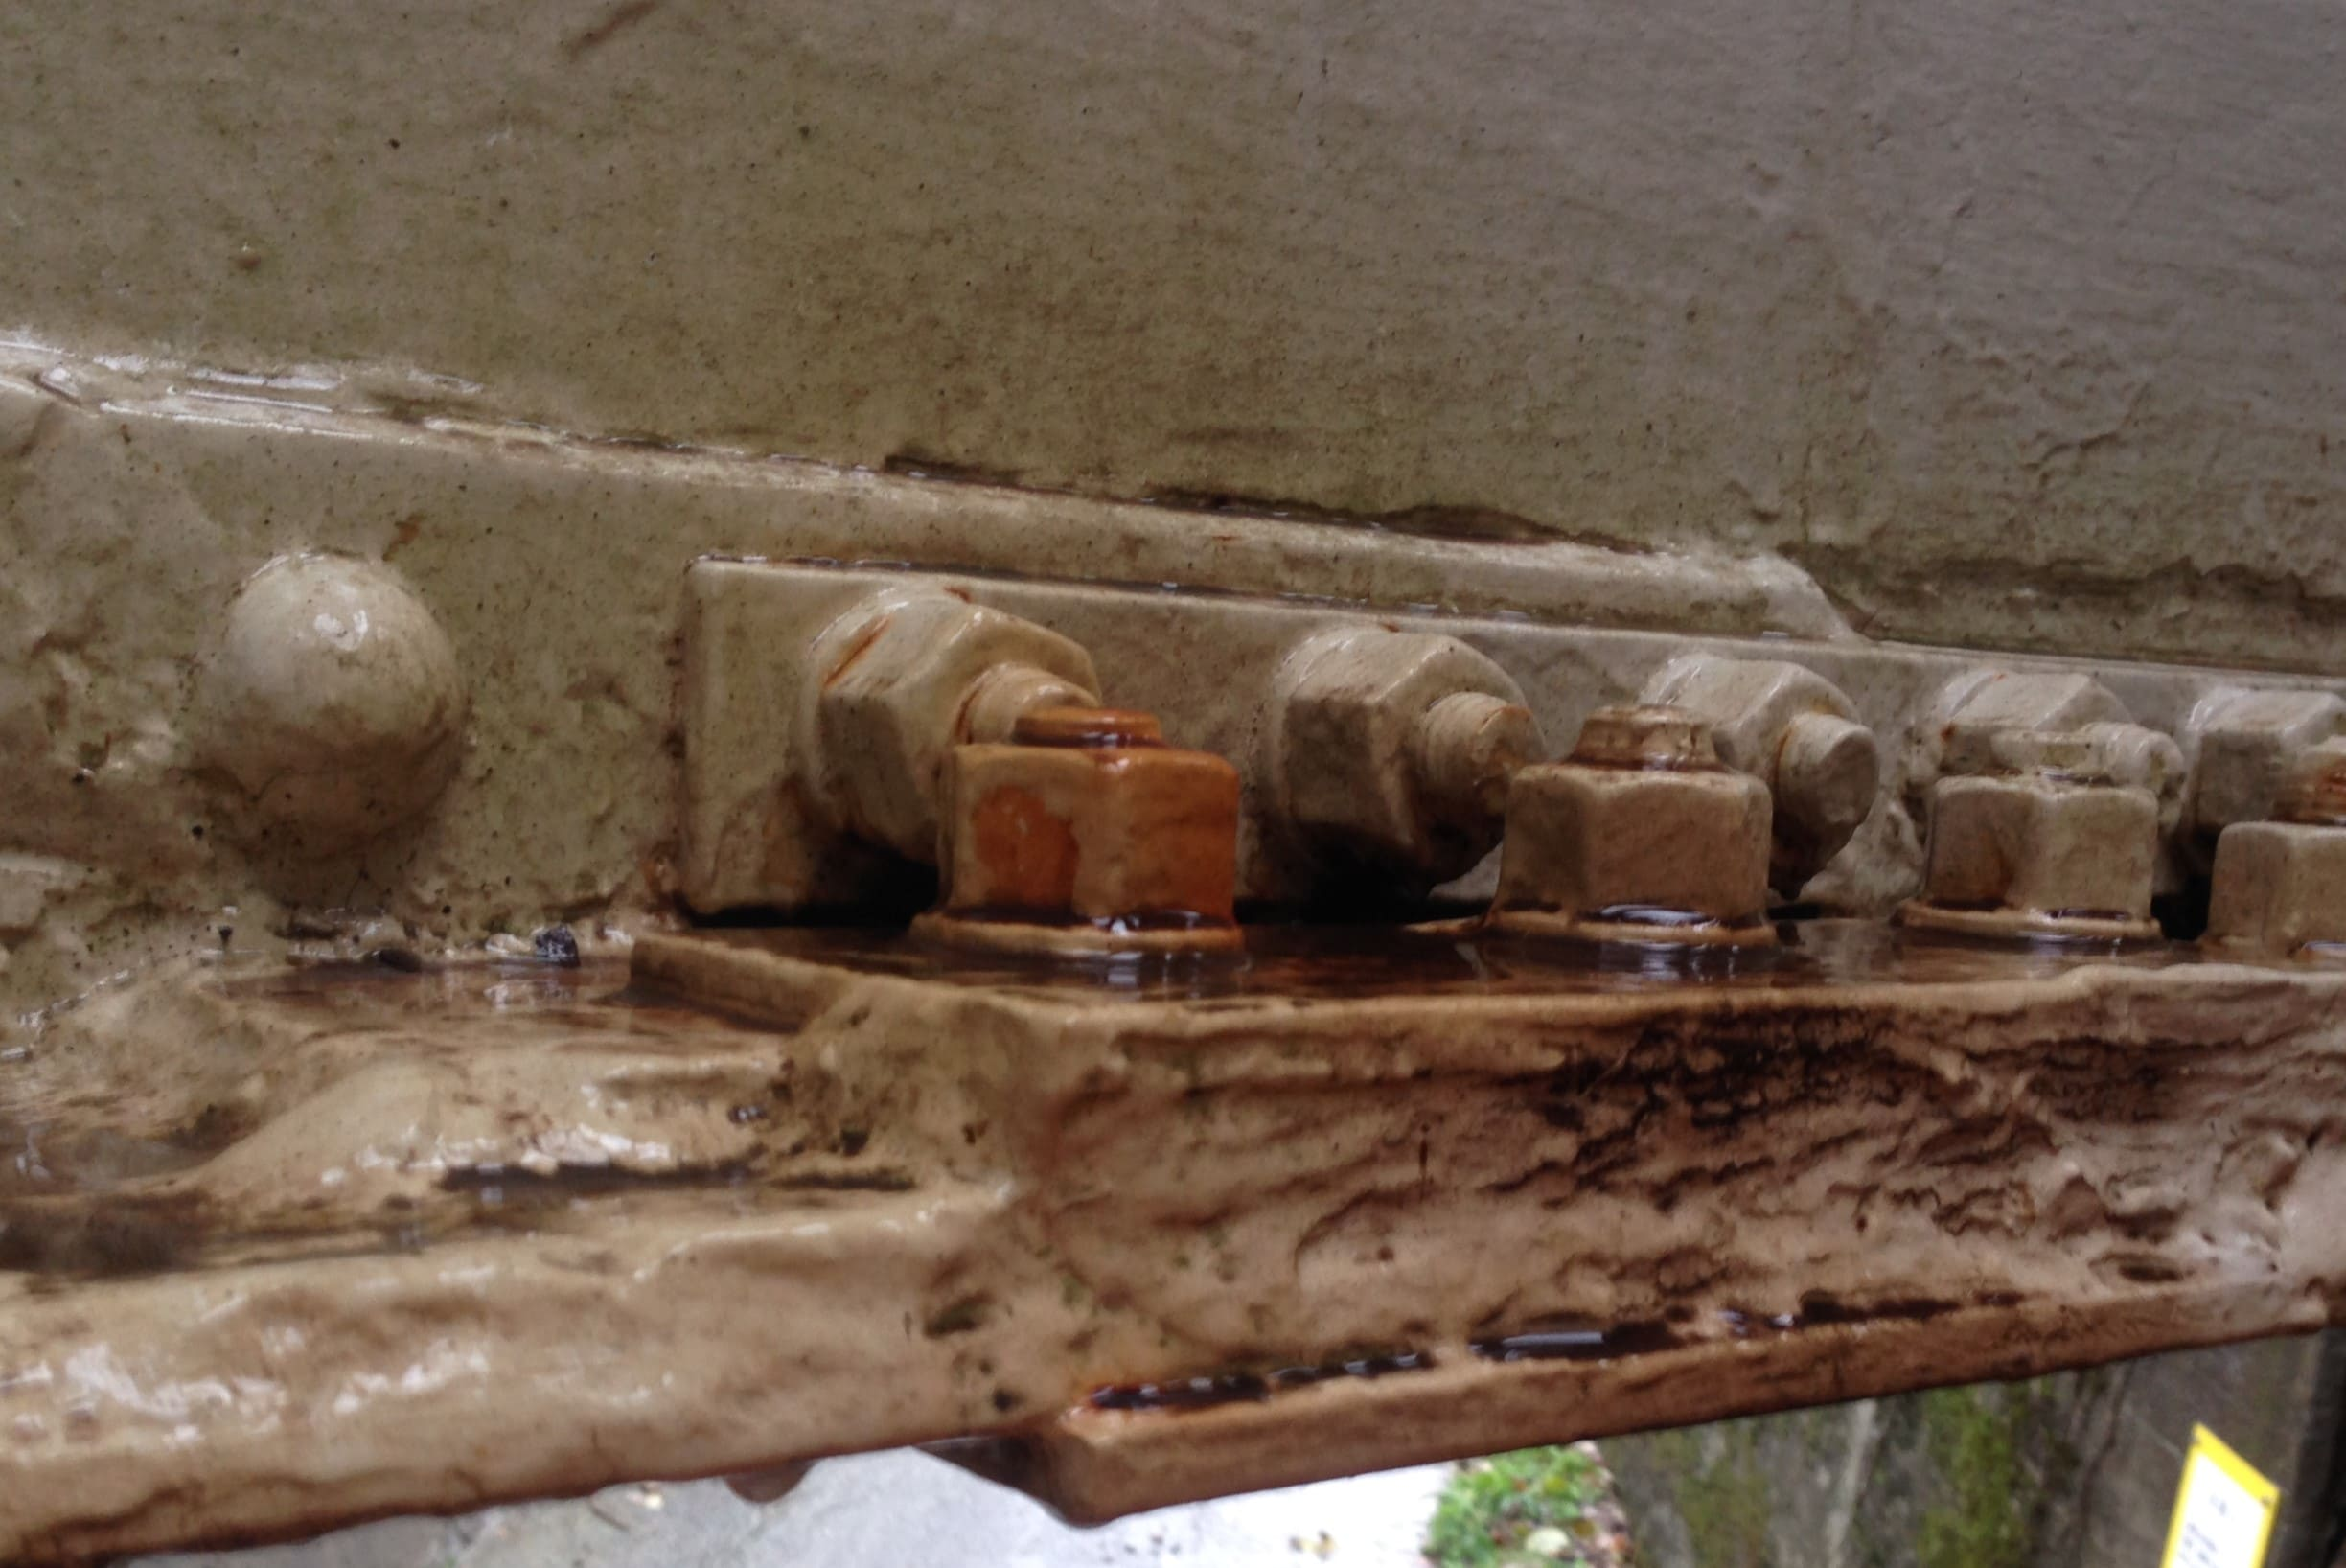
\includegraphics[width=0.75\linewidth]{imgs//ch2/bridge-rivet-HSB.jpg}
    \caption{Riveted joint combined with high-strength bolts. (Hazukawa riveted bridge, Fukui, Japan)}
    \label{fig-bridrivhsb}
\end{figure}

%This scenario may arise when reinforcing or fortifying an existing joint. For instance, it may be viable to replace several rivets with high-strength bolts. Alternatively, when there is limited space for additional fasteners, welds may be added to the joint. In both cases, the applied loads are transferred across a common shear plane using both types of fasteners. Combination joints that employ fasteners on a shared shear plane have the benefit of being compact. 

%Reducing the required space and amount of splice material, welded connections can also assist in overcoming erection problems. Despite being generally more compact than bolted connections, fabrication tolerances for welding are more precise and demand careful consideration of component positioning and holding.  Bolted connections with regular hole clearance (1/16") enable some relative movement between the connected parts subsequent to the initial assembly, and before the final tightening of the bolts. Thus, it is more convenient to employ bolts to install a member in a frame. Once the member has been placed and aligned suitably, the bolts can be tightened. It is trouble-free to add welds to a connection after it has been first bolted into place (see Fig. 14.1a).
%
\begin{figure}[ht]
    \centering
    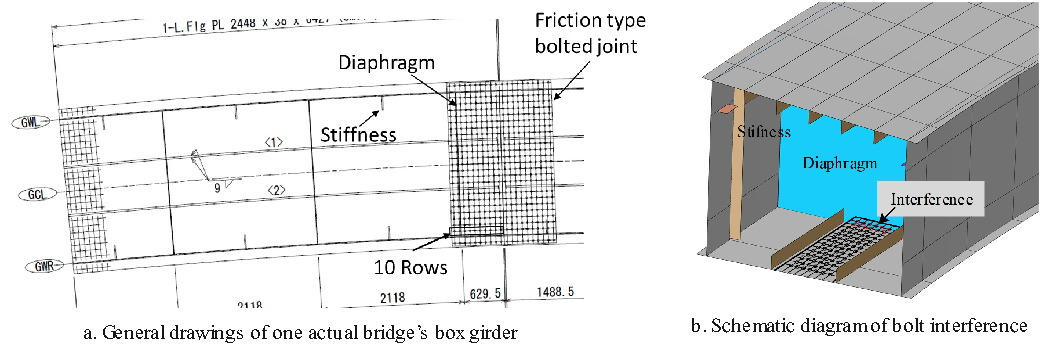
\includegraphics[width=1\linewidth]{imgs//ch2/boxhsbinter.pdf}
    \caption{Actual engineer case of the need of hybrid joint: the joint of box girder}
    \label{fig-boxhsbinter}
\end{figure}

\subsection{Rivet-HSB}

Komatsu et al.\cite{KOMATSU2015} conducted tensile load tests and chemical tests on aged steel to understand its fundamental properties. Furthermore, tensile loading tests were performed on multi-bolted joints to investigate the replacement of rivets with HSB. The test results reveal that the load carrying capacity and deformability of the partially and fully replaced HSB. joints can be enhanced by introducing frictional resistance, compared to riveted joints alone.

\begin{figure}
    \centering
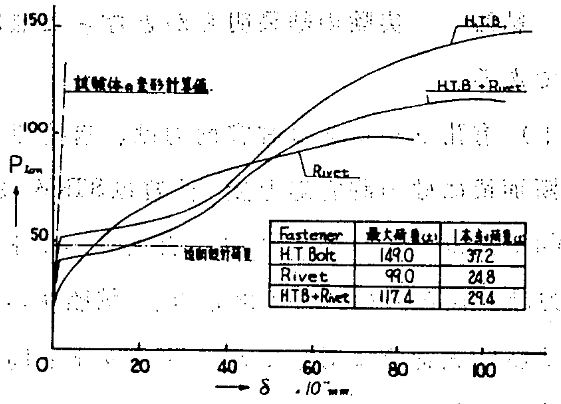
\includegraphics[width=0.5\linewidth]{imgs//ch2/hsbrivet-1967-pd.png}
    \caption{Relationship between load and deformation of Hybrid joint combined with 2 HSB and 2 rivet}
    \label{fig-hsbriv-fune}
\end{figure}
\subsection{HSB-Weld}

\subsection{HSB-IFB}

\label{sec-hsbweld}

Adding Welds to Mechanically Fastened Joints Welded connections are rigid. Welded connections are stiff. Unlike snug-tightened bolted joints that may slip as they are loaded, welds are not expected to stretch and distribute the applied load to any great extent. In most cases, welds and bearing-type mechanical fasteners will not deform equally.

When welds and mechanical fasteners are used together, load is transferred through the stiffer part; therefore, the weld can carry almost all the load, sharing little with the bolts. That is why caution needs to be taken when welds, bolts, and rivets are combined.Code Provisions. The issue of mixing mechanical fasteners and welds is addressed in AWS D1. 1:2000 Structural Welding Code—Steel. Provision 2.6.3 states that for rivets or bolts used in bearing-type connections (that is, when the bolt or rivet acts as a pin), the mechanical fasteners shouldn't be considered as sharing the load in combination with welds. If welds are used, they should be provided to carry the entire load in the connection. However, connections that are welded to one member and riveted or bolted to another are permitted.

%https://www.thefabricator.com/thefabricator/article/arcwelding/mixing-welds--bolts
%https://pressbooks.bccampus.ca/powr4406/chapter/bolted-and-welded-joints/

\section{Regulations and standards}

\subsection{Riveted joint}

Shear resistance, per shear plane, Eurocode:
\begin{equation}
F_{\mathrm{v}, \mathrm{Rd}}=\frac{0,6 f_{\mathrm{ur}} A_0}{\gamma_{\mathrm{M} 2}}
\end{equation}